\title{Lecture 14\\Fundamental Principles for Developing Semantic Models of Knowledge Bases}

\begin{frame}
	\titlepage
\end{frame}

\begin{frame}{\\Lecture outline}
	\topline
	\justifying
	The methodology and main stages of knowledge base development. Identifying a hierarchy of subject domains. Developing ontologies.
\end{frame}

\begin{frame}{Knowledge base development methodology}
	\topline
	\justifying

	Research on knowledge base development methods focuses primarily on how to develop \textbf{\textit{ontologies}}, a core component of modern knowledge bases.

	An ontology development methodology provides instructions and guidelines for carrying out the complex procedures involved. It specifies the tasks, how and in what order to perform them, and how to document the work.
\end{frame}

\begin{frame}{Stages of hybrid knowledge base development}
	\topline
	\justifying
	\vspace{8mm}
	\begin{textitemize}
		\item Define the initial structure of the hybrid knowledge base.
		\item Identify components that can be taken from a library of reusable knowledge base components and incorporate them into the new knowledge base.
		\item Specify the work needed to develop the missing parts of the knowledge base and assign it to the developers.
		\item Develop and agree on the new parts. These may later be added to the library of reusable knowledge base components.
		\item Verify and debug the knowledge base.
	\end{textitemize}
\end{frame}

\begin{frame}{Knowledge base development for OSTIS systems}
	\topline
	\justifying
	\vspace{8mm}
	\begin{textitemize}
		\item Identify the system's goals and the tasks it must perform.
		\item Define a hierarchy of subject domains based on those tasks.
		\begin{textitemize}
			\item Define the knowledge field: a preliminary set of all concepts that may appear in the knowledge base.
			\item Make an initial assignment of concepts to subject domains.
			\item Reuse existing components from the \textbf{\textit{OSTIS Metasystem}}, such as the subject domains of sets, relations, parameters, numbers, and logical formulas.
		\end{textitemize}
		\item Specify each subject domain by defining its system of concepts.
		\item Build a family of ontologies for each subject domain.
		\item Describe instances of the concepts in each subject domain.
	\end{textitemize}
\end{frame}

\begin{frame}{\\Knowledge base section}
	\topline
	\justifying
	\vspace{8mm}

	A knowledge base section is a logically distinct part of a knowledge base, organized so that people, including end users and developers, can understand and analyze it.
	\bigskip

	Why introduce sections?
	\begin{textitemize}
		\item Some knowledge base content cannot conveniently be assigned to a subject domain.
		\item The subject domain \underline{does not include} its ontology.
	\end{textitemize}
\end{frame}

\begin{frame}{\\Knowledge base section}
	\topline
	\justifying
	\vspace{8mm}
	\begin{SCn}
		\scnheader{knowledge base section}
		\scnsubset{structure}
		\begin{scnrelfromset}{partition}
			\scnitem{atomic section}
			\scnitem{non-atomic section}
		\end{scnrelfromset}
	\end{SCn}

	A non-atomic section can be decomposed into subsections.

	\begin{SCn}
		\scnheader{knowledge base section}
		\scnsuperset{subject domain and ontology section}
		\scnsuperset{knowledge base structure section}
		\scnsuperset{\dots}
	\end{SCn}
\end{frame}

\begin{frame}{\\Example of a knowledge base section}
	\topline
	\justifying
	\vspace{8mm}
	\begin{SCn}
		\scnheader{Section: Subject domain of geometric figures}
		\scnsubset{structure}

		\begin{scnrelfromset}{section decomposition}
			\scnitem{Section: Subject domain of polygons}
			\scnitem{Section: Subject domain of circles}
		\end{scnrelfromset}
		\scniselement{non-atomic section}
	\end{SCn}
\end{frame}

\begin{frame}{\\Example of a knowledge base section}
	\topline
	\justifying
	\vspace{7mm}
	\begin{figure}
		\centering
		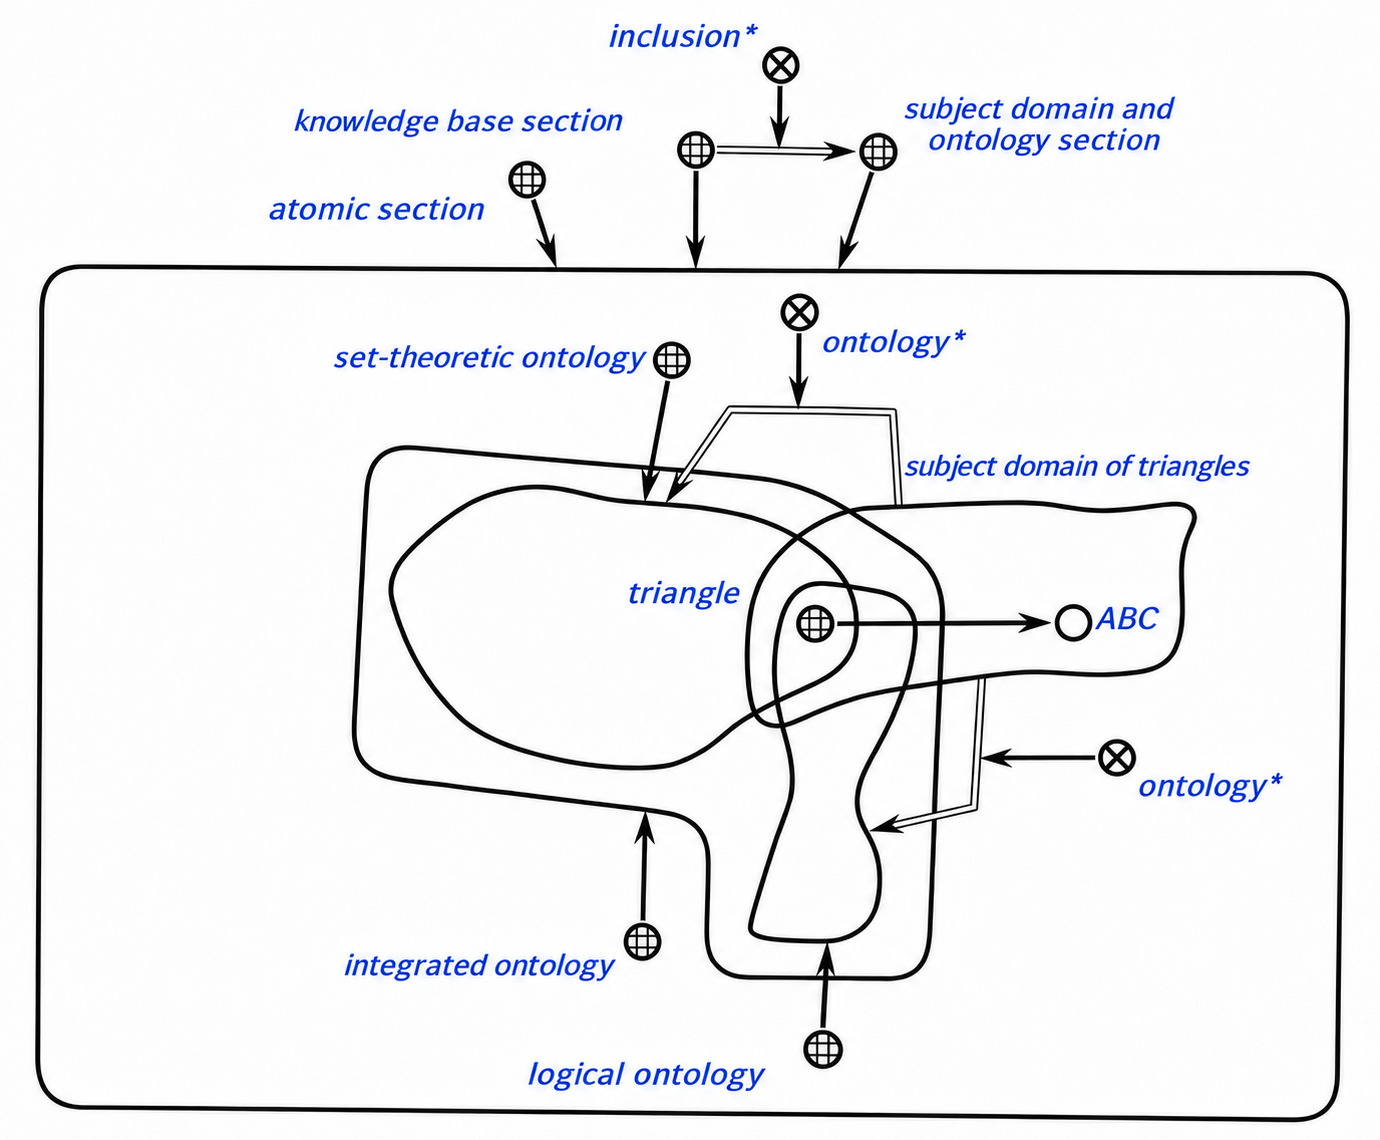
\includegraphics[width=\linewidth,height=0.71\textheight,keepaspectratio]{figures/kb_develop_principles/example_en.png}
	\end{figure}
\end{frame}

\begin{frame}{\\How to introduce a new subject domain}
	\topline
	\justifying
	\vspace{8mm}
	\begin{textitemize}
		\item Identify the higher-level subject domain or domains of which the new domain will be a child, based on the class of objects of study and on the relations under study.
		\item Develop a structural specification.
		\item Develop a system of concepts.
		\item Develop examples.
	\end{textitemize}
	\bigskip
	The following are generally specified explicitly:
	\begin{textitemize}
		\item The subject domain and its structural specification.
		\item The subject domain and ontology section and its contents.
	\end{textitemize}
\end{frame}

\begin{frame}{\\How to introduce a new concept}
	\topline
	\justifying
	\vspace{8mm}
	\begin{textitemize}
		\item Identify the nearest superclass (the closest more general concept).
		\item Identify the subject domain for the concept, introducing a new one if necessary.
		\item Develop a terminological specification.
		\item Develop a set-theoretic specification.
		\item Develop a logical specification in both natural language and SCL.
	\end{textitemize}
\end{frame}
